% Key figures only; every other figure is in the repository's figures/ folder.
More figures (training curves, every seed, memory, per-task and per-error breakdowns, drift, Part B, the full C1 grid, example outputs) are in \texttt{figures/} of the repository.

\begin{figure}[H]
\centering
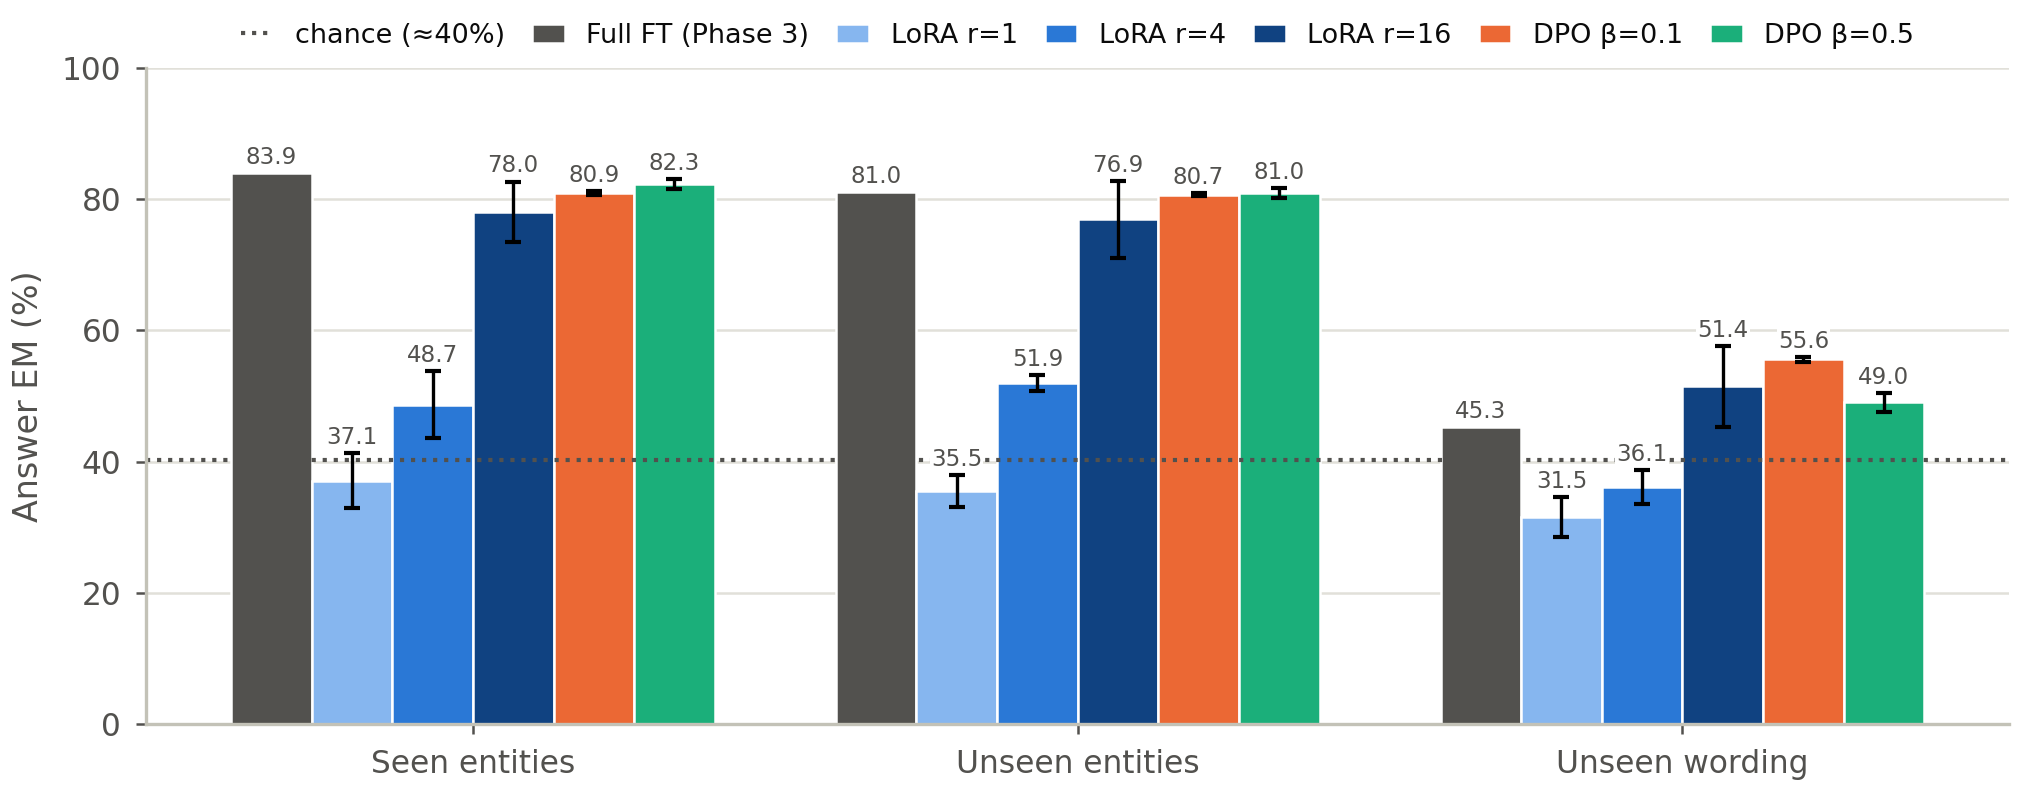
\includegraphics[width=\textwidth]{../figures/fig_ada_main.png}
\caption{A2/A4: answer EM on the three test sets. Full FT: the Phase 3 checkpoint; LoRA and DPO (chosen configuration): mean $\pm$ sd over 3 seeds. Dotted line: chance.}
\label{fig:sweep}
\end{figure}

\begin{figure}[H]
\centering
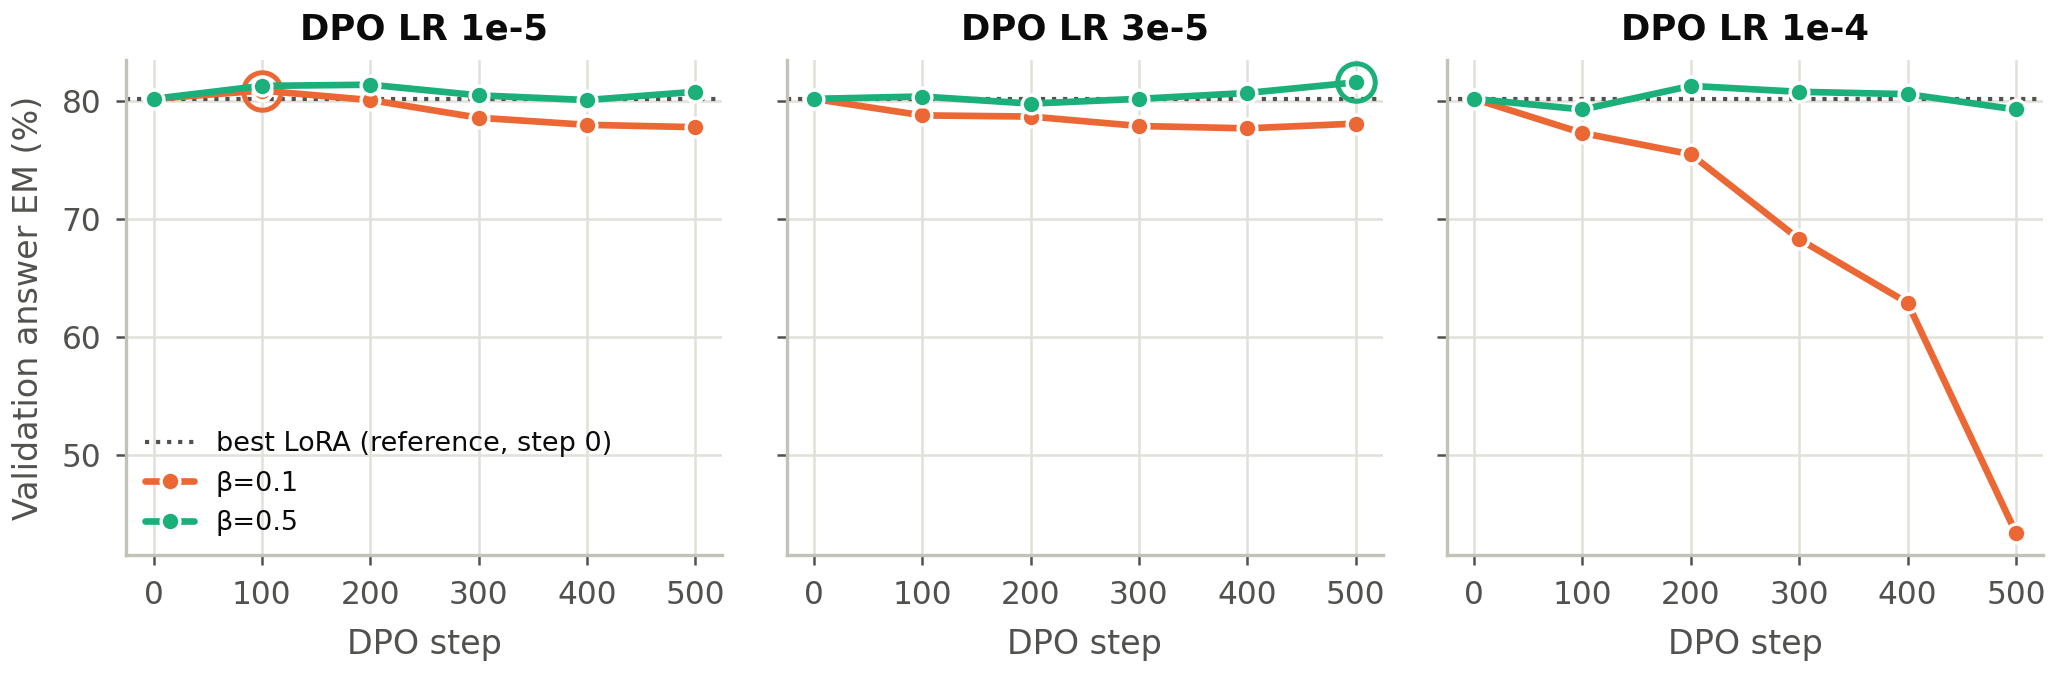
\includegraphics[width=\textwidth]{../figures/fig_a4_dpo_sweep_val.png}
\caption{A4: DPO sweep (seed 42). Validation answer EM of the policy saved every 100 steps, for each LR and both $\beta$; step 0 is the best LoRA model (dotted); the ring marks the configuration chosen for each $\beta$.}
\label{fig:dposweep}
\end{figure}

\begin{figure}[H]
\centering
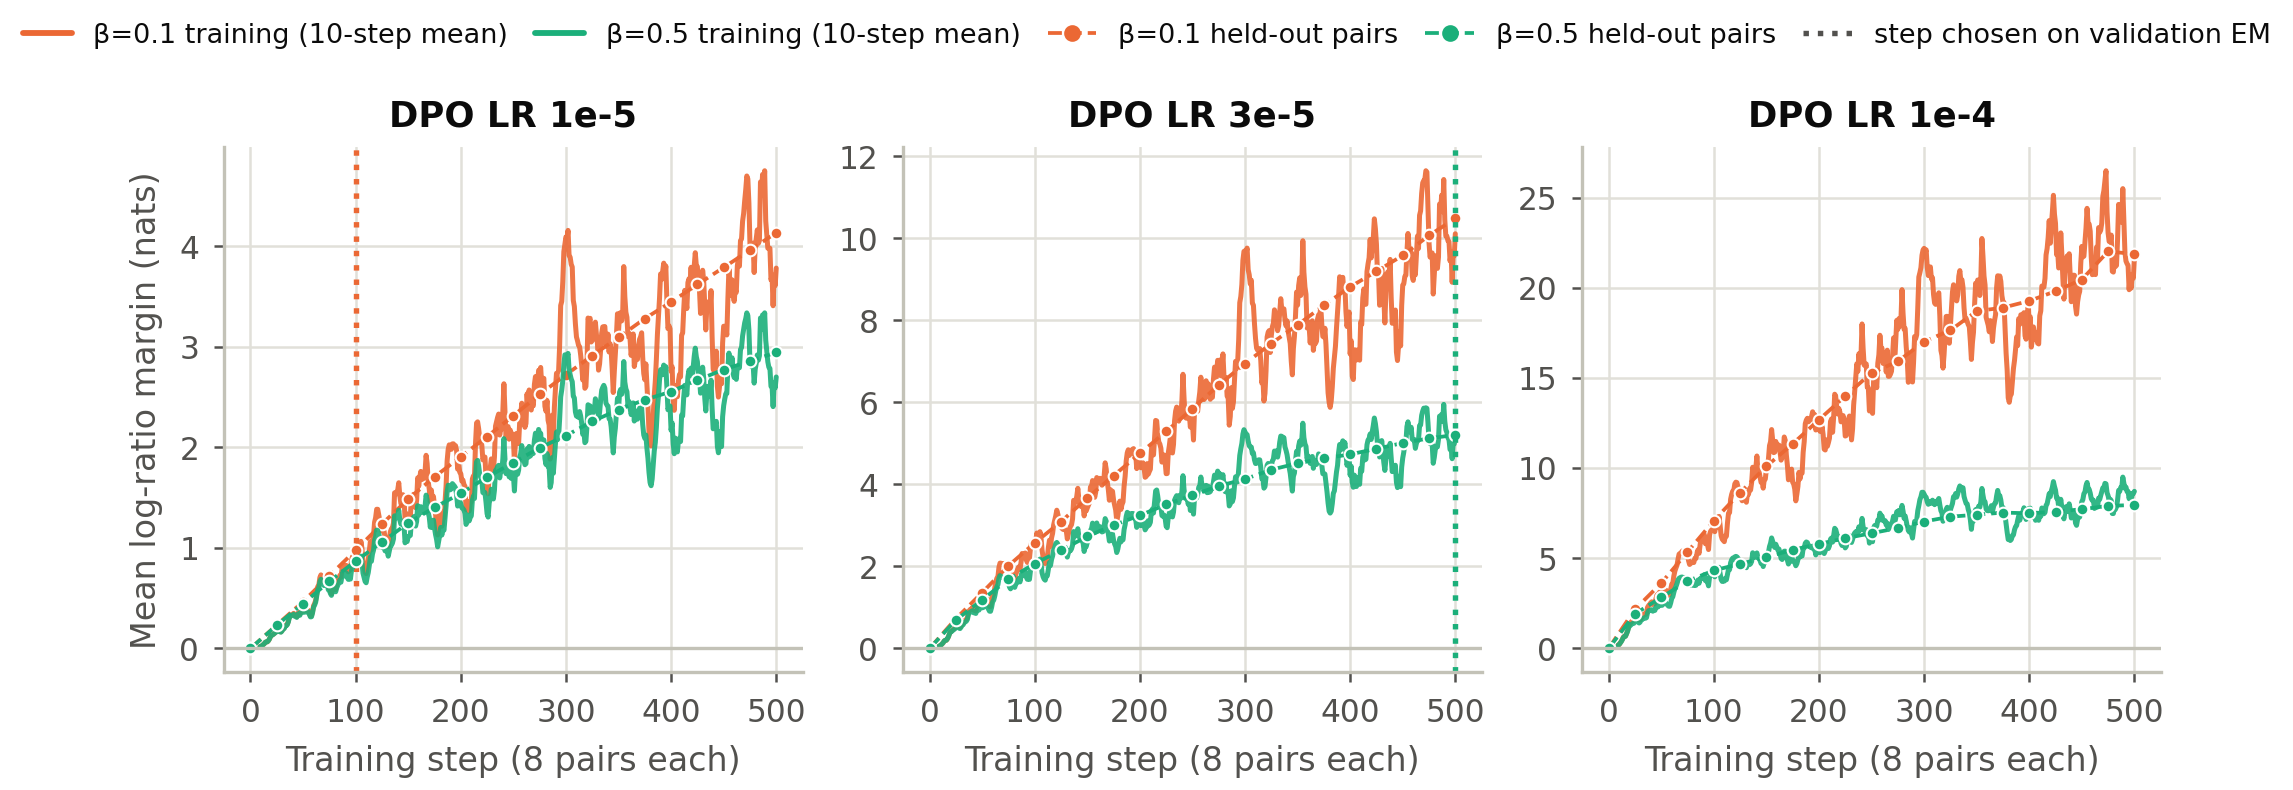
\includegraphics[width=\textwidth]{../figures/fig_ada_dpo_margins.png}
\caption{A4: mean chosen-minus-rejected log-ratio margin over DPO training for $\beta=0.1$ and $\beta=0.5$, at each LR (seed 42). Solid: training batches (10-step mean); dashed: the 400 held-out validation pairs; dotted vertical: the step chosen on validation accuracy.}
\label{fig:dpo}
\end{figure}

\begin{figure}[H]
\centering
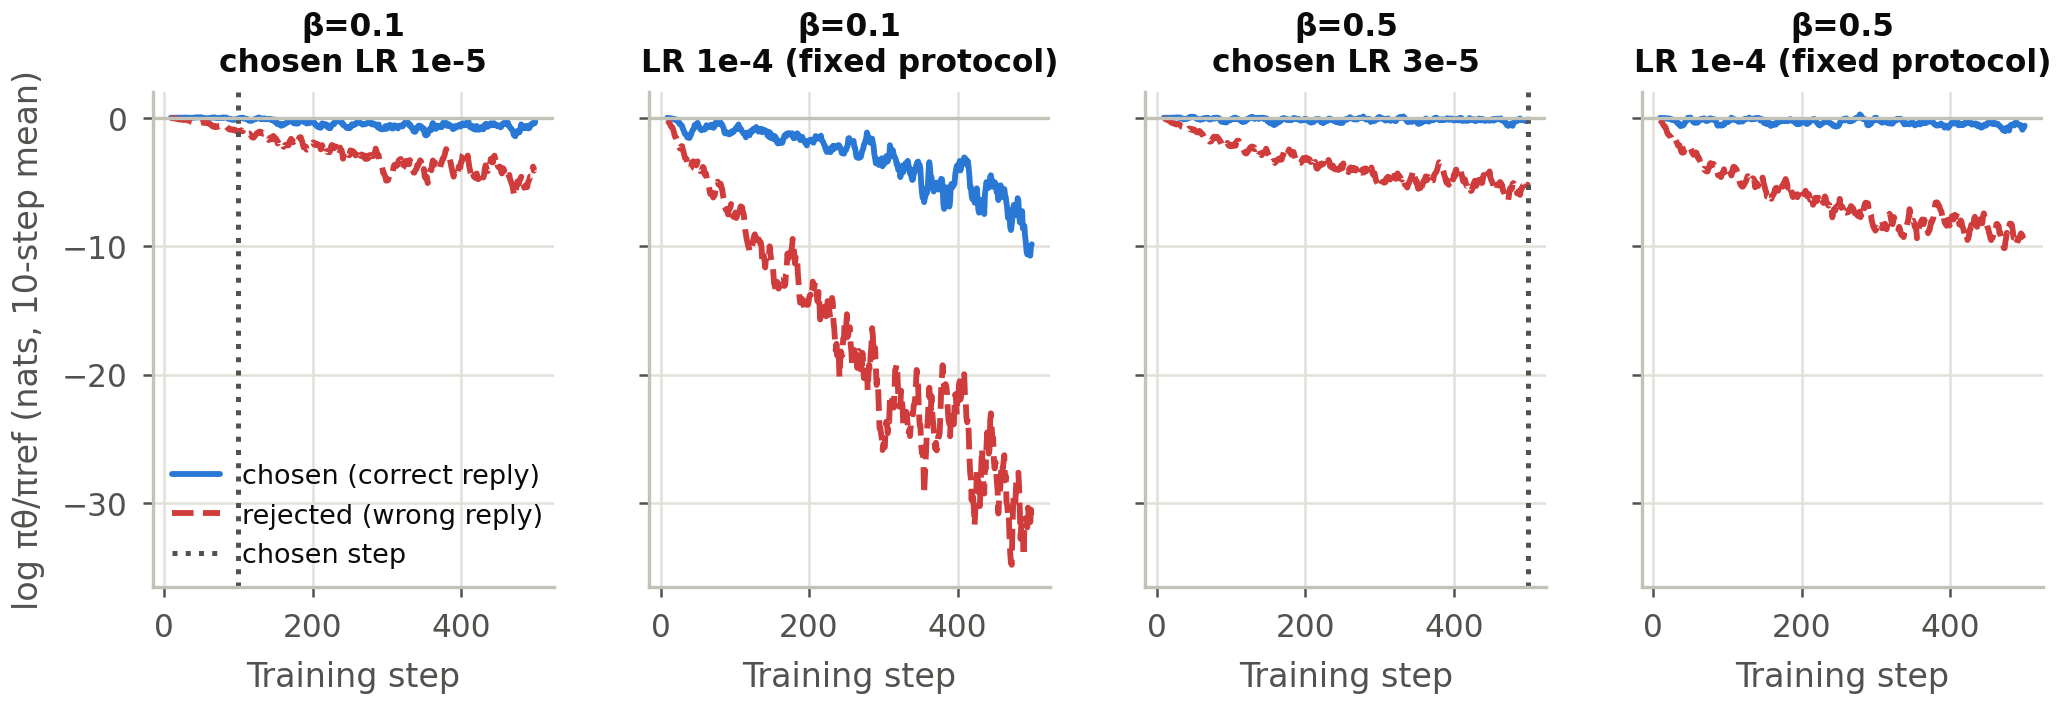
\includegraphics[width=\textwidth]{../figures/fig_ada_dpo_logratios.png}
\caption{A4: log-ratios $\log\pi_\theta/\pi_{\rm ref}$ of the chosen (correct) and the rejected (wrong) replies separately (seed 42), for each $\beta$'s chosen LR and for the fixed protocol (LR $10^{-4}$).}
\label{fig:logratios}
\end{figure}

\begin{figure}[H]
\centering
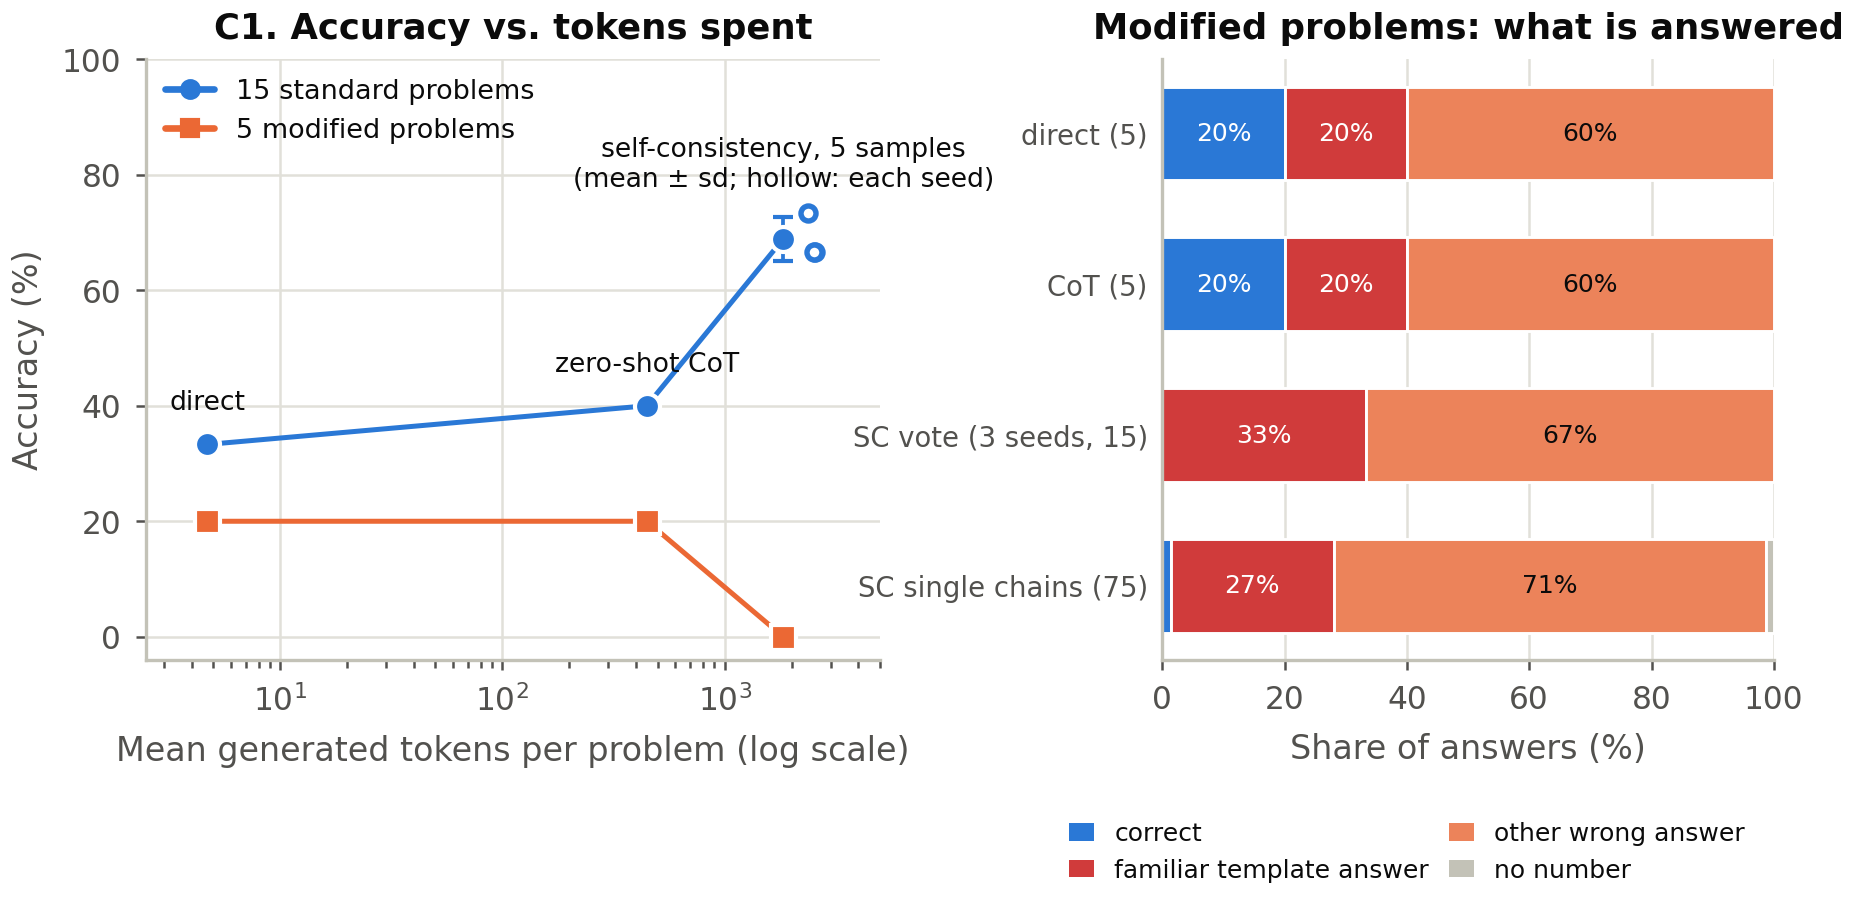
\includegraphics[width=\textwidth]{../figures/fig_eval_c1_tokens.png}
\caption{C1. \emph{Left:} accuracy against mean generated tokens per problem (log scale). Thinking longer helps on the 15 standard problems but not on the 5 modified ones: direct and CoT each solve one (M02 and M05), voting none. \emph{Right:} what the model answers on the modified problems: mostly another wrong number, and the familiar template's answer in a fifth to a third of the answers (such as 8 for ``all except 9''). One of the 75 sampled chains is right (M05); no vote is.}
\label{fig:c1tokens}
\end{figure}

\begin{figure}[H]
\centering
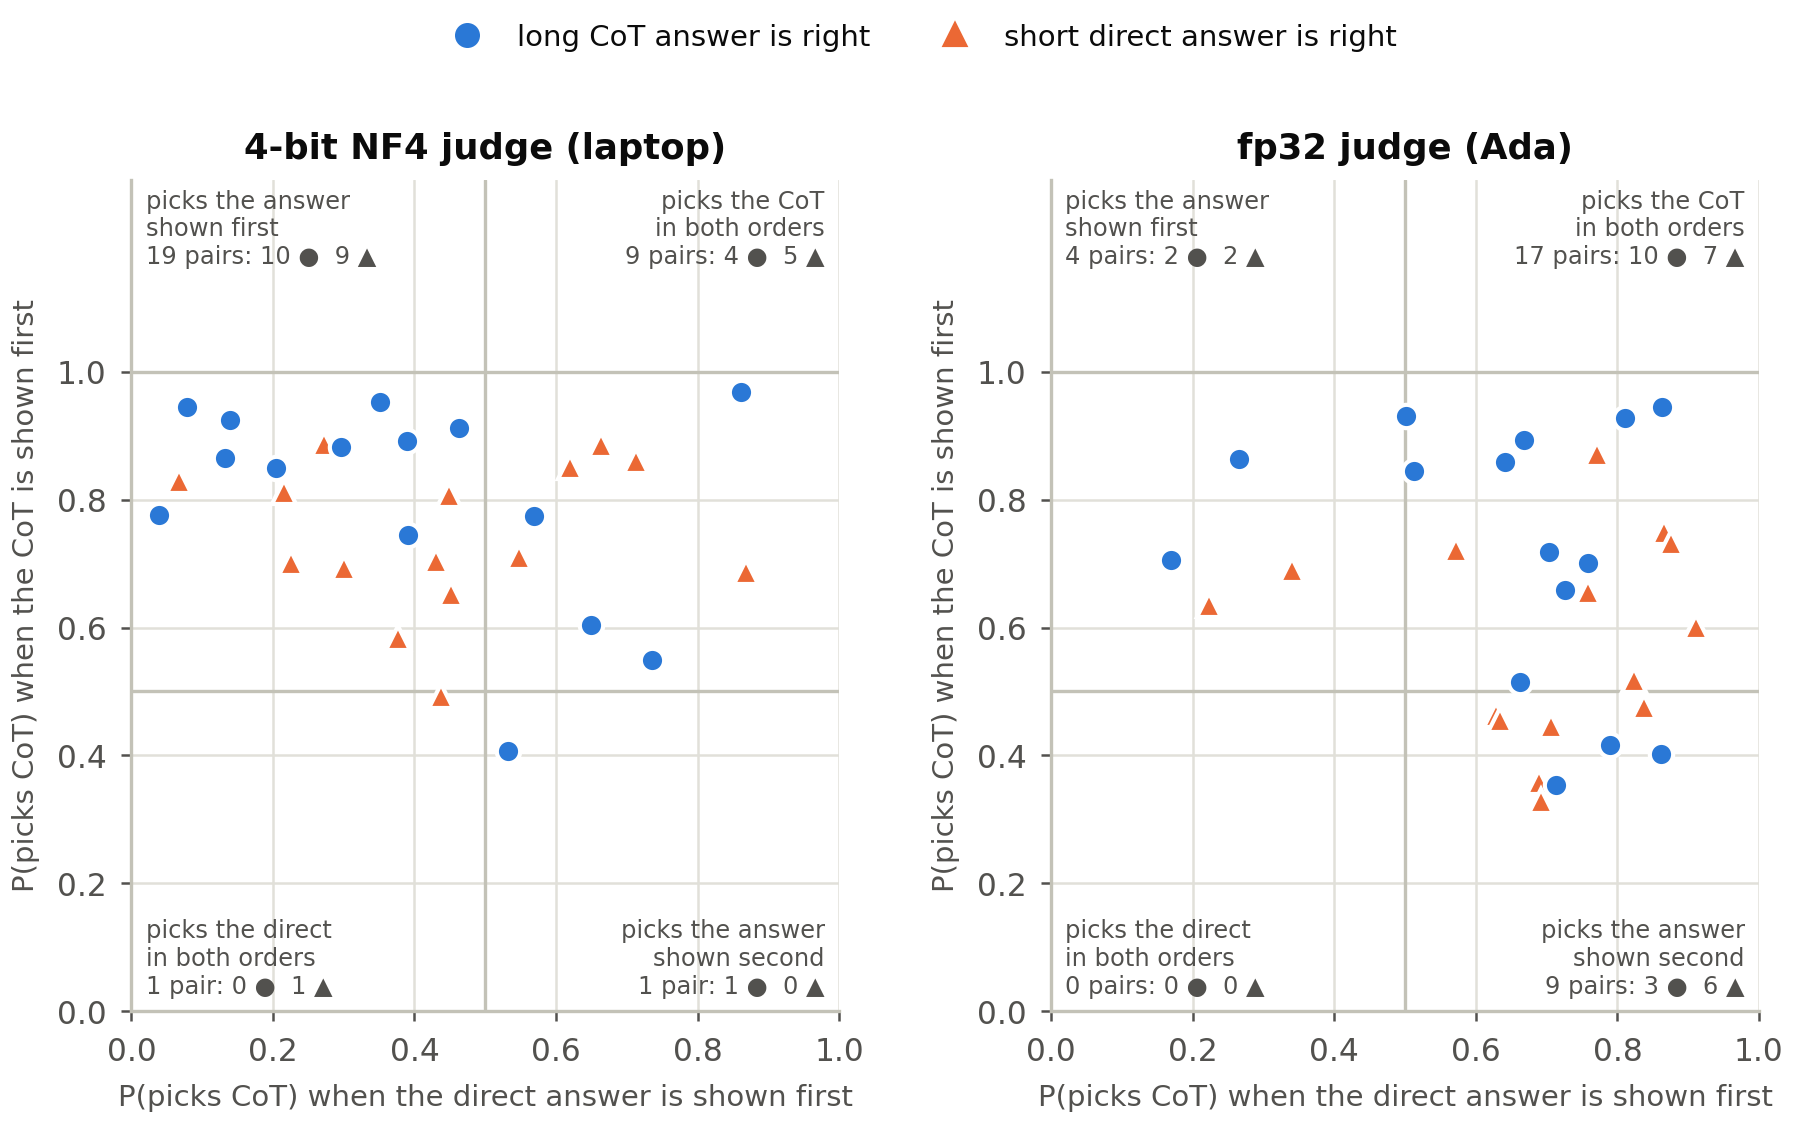
\includegraphics[width=\textwidth]{../figures/fig_eval_c2_judge.png}
\caption{C2: each of the 30 pairs, placed by the judge's probability of preferring the CoT reply when the direct reply is shown first ($x$) and when the CoT reply is shown first ($y$). The top-left and bottom-right quadrants are order flips. Counts: \textbullet\ pairs where the CoT reply is right, $\blacktriangle$ pairs where the direct reply is right. The 4-bit judge sits mostly top-left (it picks the first answer shown; \CTwoPosBiasN\ of 30 pairs flip). The fp32 judge sits mostly top-right (it picks the long CoT in both orders in \FpConsistent\ pairs, right or not; \FpPosBiasN\ flip). A judge that read for correctness would put \textbullet\ top-right and $\blacktriangle$ bottom-left.}
\label{fig:c2judge}
\end{figure}
